\documentclass[letterpaper,10pt,conference]{ieeeconf}

\usepackage{graphicx}
\usepackage{amsmath}
\usepackage{float}

\title{Medial Axis Detection of Moving Objects}

\author{Adari Harshit(25CH10029)}

\begin{document}

\maketitle

\begin{abstract}

This report presents a method to detect the medial axis of a moving tool in video data. 
The input videos are processed frame by frame. A background subtraction method is first used to isolate the moving object. 
The resulting mask contains noise and small artifacts. Median filtering and morphological operations are applied to clean the image. 
Edge boundaries of the tool are then extracted using the Canny edge detector. 
A custom implementation of the Hough Transform is used to detect straight lines corresponding to the tool edges. 
Two nearly parallel lines are selected from the detected lines. 
The midpoint between these lines is computed to estimate the medial axis. 
The detected axis is drawn on the original frame for visualization. 
The method was tested on three input videos. 
The results show that the approach is able to track the central axis of the tool across frames.

\end{abstract}


\section{INTRODUCTION}

Computer vision helps machines understand images and videos. 
Many robotics systems use cameras to observe objects and their motion. 
Visual information is often used for tracking and navigation.

One useful representation of an object is its medial axis. 
The medial axis is the center line of a shape. 
It describes the orientation and structure of elongated objects.

In this task, the goal is to detect the medial axis of a moving surgical tool. 
The input is a set of video clips containing the tool. 
Each video must be processed frame by frame.

The processing follows a sequence of image operations. 
First, the moving object is separated from the background. 
The resulting mask contains noise and small artifacts. 
Image cleaning is applied to improve the silhouette of the tool.

Edges of the cleaned object are then detected. 
Straight edges of the tool are identified using the Hough Transform. 
Finally, the midpoint between two parallel edges is computed. 
This midpoint represents the medial axis of the tool.

The detected medial axis is drawn on the original frame for visualization.


\section{PROBLEM STATEMENT}

The objective of this task is to detect the medial axis of a moving surgical tool from video data. 
Three video clips are provided as input. 
Each video contains a thin tool moving across the scene.

The algorithm must process the video frames and identify the central axis of the tool. 
The detected axis should be drawn on the original video frame.

The solution must follow a defined processing pipeline. 
First, the moving object must be separated from the background using background subtraction. 
This step produces a foreground mask of the tool.

The resulting mask may contain noise and irregular regions. 
Morphological image processing techniques are used to clean the image and improve the object silhouette.

After cleaning, edges of the tool must be detected. 
Straight edges of the object must then be identified using the Hough Line Transform.

Using the detected edges, the midpoint between two parallel lines is computed. 
This midpoint represents the medial axis of the tool.

The final output is the original video frame with the medial axis highlighted.

\section{RELATED WORK}

Several image processing techniques are commonly used to detect object structure in images. 
Edge detection and line detection are widely used in computer vision applications.

The Canny edge detector is a popular method for identifying object boundaries. 
It detects strong intensity gradients in an image and produces a thin edge map. 
This method is commonly used before performing line detection.

The Hough Transform is widely used for detecting straight lines in images. 
OpenCV provides a built-in implementation through the \texttt{cv2.HoughLines()} and \texttt{cv2.HoughLinesP()} functions. 
These functions detect straight lines by transforming edge points into a parameter space representation.

Several tutorials and documentation resources were used to understand these techniques. 
OpenCV documentation provides explanations of background subtraction, morphological operations, and edge detection \cite{opencv_docs}. 
Educational tutorials and examples also helped in understanding practical implementation using Python and OpenCV \cite{gfg_opencv}. 
Video lectures were also used to study the theory behind image processing and the Hough Transform \cite{yt_cv_course, yt_opencv_video}.

In this project, the OpenCV functions were used for basic image processing operations such as filtering, morphological cleaning, and edge detection. 
However, the Hough Transform for line detection was implemented manually in order to understand the algorithm and follow the task requirements.


\section{METHODOLOGY}

The algorithm processes the video frame-by-frame and extracts structural features of the moving tool. 
The overall pipeline used in this work is shown below:

\begin{center}
Video Frames $\rightarrow$ Background Subtraction $\rightarrow$ Image Cleaning $\rightarrow$ Edge Detection $\rightarrow$ Hough Line Detection $\rightarrow$ Medial Axis
\end{center}


\subsection{Background Subtraction}

The first step involves isolating the moving foreground object from the static background. 
This is achieved using the Gaussian Mixture Model based background subtraction technique implemented in OpenCV 
(\texttt{cv2.createBackgroundSubtractorMOG2}). 

The output of this stage is a binary mask where the foreground object appears in white while the background remains black.


\subsection{Image Cleaning}

The binary mask obtained from background subtraction contains noise and small artifacts. 
To improve the silhouette of the object, morphological operations are applied.

First, a median filter is used to reduce salt noise. 
Then morphological opening and closing operations are applied using rectangular structuring elements. 
Opening removes isolated noise pixels while closing fills small gaps in the object boundary.

These operations produce a cleaner representation of the tool.


\subsection{Edge Detection}

After cleaning the mask, edges of the object are detected using the Canny edge detector. 
The Canny algorithm computes image gradients and identifies strong intensity transitions corresponding to edges.

The parameters used include a lower threshold of 50, an upper threshold of 150, and an aperture size of 3 with the L2 gradient option enabled. 
The resulting image contains clear edge boundaries corresponding to the sides of the tool.


\subsection{Custom Hough Line Transform}

To detect the straight edges of the tool, the Hough Line Transform is implemented from scratch. 
The algorithm transforms edge pixels from image space into the $(\rho,\theta)$ parameter space using the equation

\[
\rho = x\cos\theta + y\sin\theta
\]

For each edge pixel, votes are accumulated in a 2D accumulator array representing possible lines. 
Peaks in this accumulator correspond to prominent straight lines in the image.

Unlike the built-in OpenCV implementation, this approach manually computes the accumulator and identifies line candidates.


\subsection{Medial Axis Computation}

Once the straight edges of the tool are detected, two nearly parallel lines are selected. 
The medial axis is computed as the average of these lines in the Hough parameter space:

\[
\rho_{mid} = \frac{\rho_1 + \rho_2}{2}, \qquad
\theta_{mid} = \frac{\theta_1 + \theta_2}{2}
\]

This midpoint line represents the central axis of the tool. 
Finally, the detected medial axis is drawn on the original video frame for visualization.


\section{RESULTS AND OBSERVATIONS}

The proposed pipeline was tested on three video sequences containing a moving surgical tool. 
Each video was processed frame by frame using the implemented pipeline. 
Intermediate outputs were recorded to examine the behavior of each stage.

Figure~\ref{fig:pipeline1} shows the processing stages for Video 1. 
The first image shows the input frame extracted from the video. 
Background subtraction isolates the moving tool and produces a binary mask. 
Some noise appears in this mask due to small intensity changes in the scene.

The image cleaning stage reduces this noise. 
Median filtering and morphological operations improve the silhouette of the tool. 
The cleaned image provides a clearer representation of the object.

Edge detection is then applied to the cleaned image. 
The Canny detector highlights the boundaries of the tool. 
Two strong edges corresponding to the sides of the tool can be observed.

The custom Hough Transform identifies straight lines along these edges. 
Two nearly parallel lines are selected from the detected candidates. 
The midpoint between these lines is computed to estimate the medial axis.

The final image shows the detected medial axis drawn on the original frame. 
The axis follows the orientation of the tool and remains close to its center.

\begin{figure}[H]
\centering

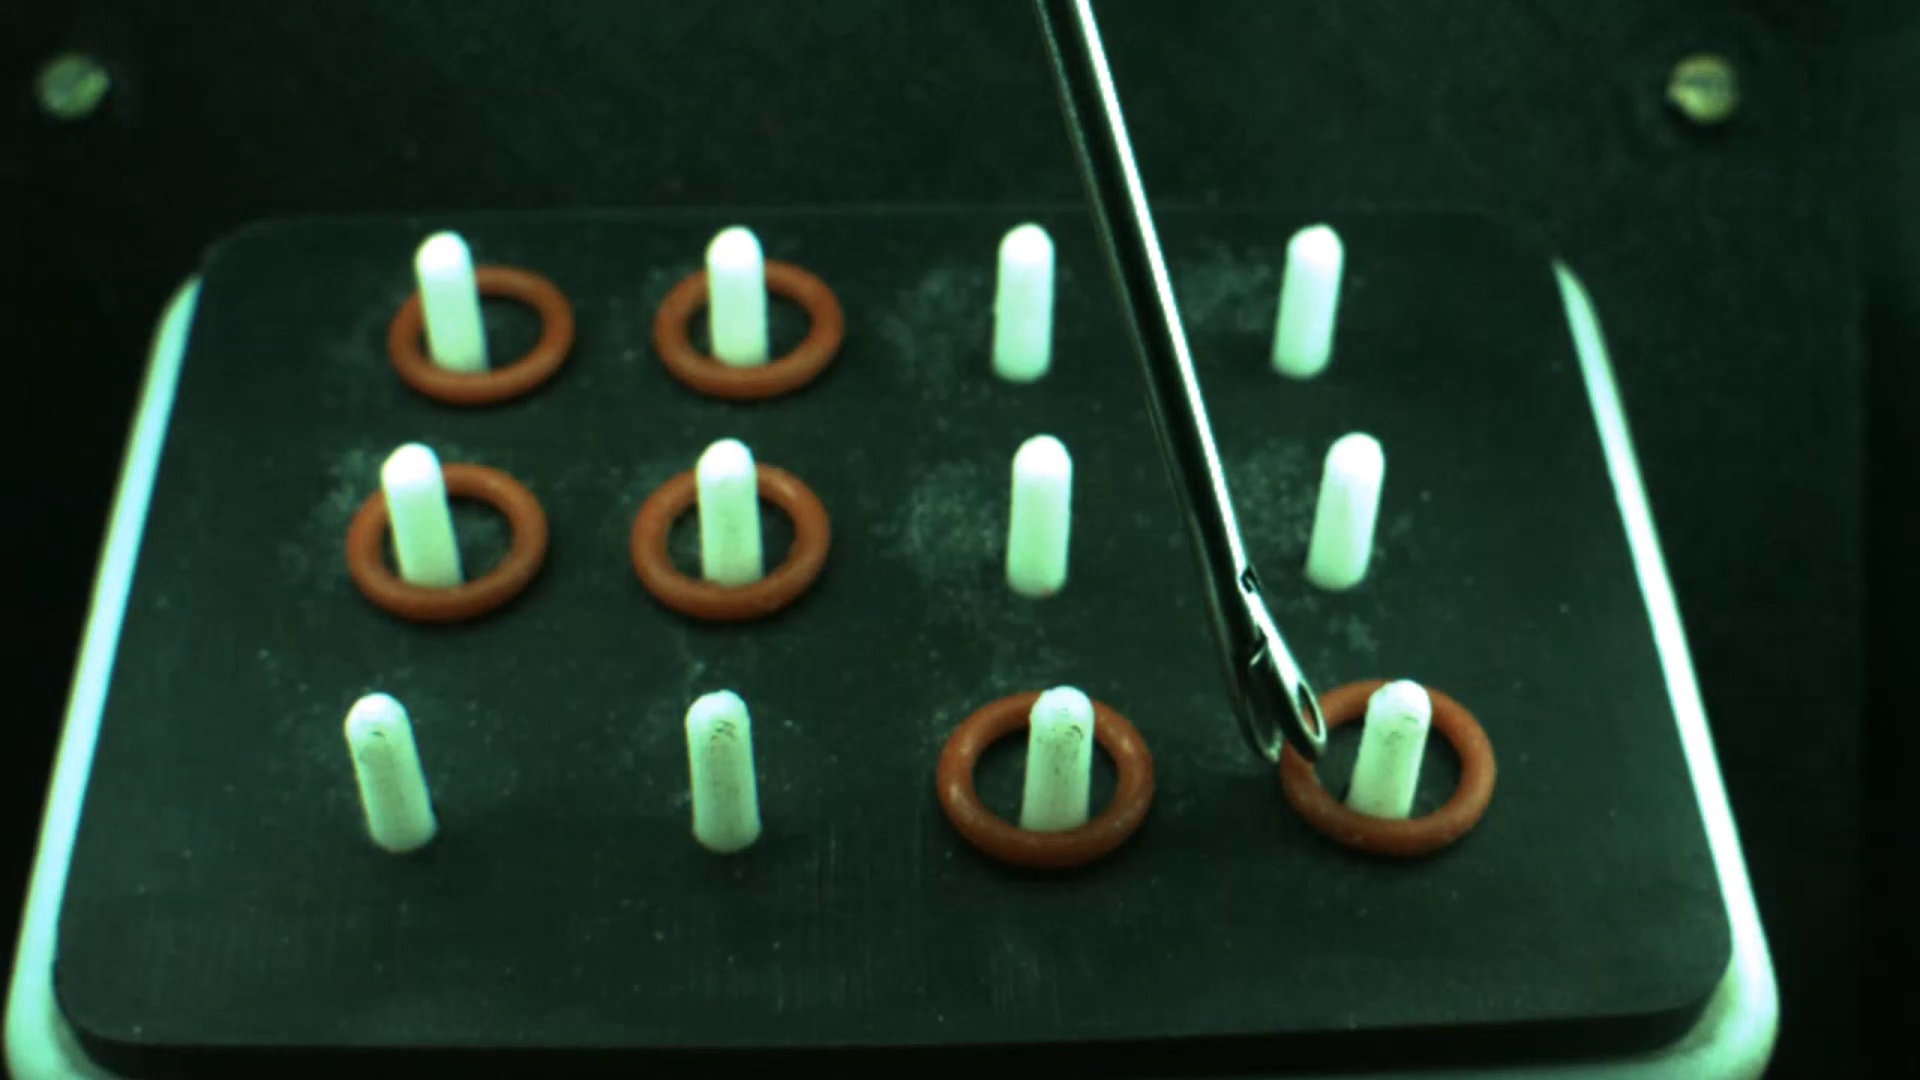
\includegraphics[width=0.45\linewidth]{results/frames/1_input.jpg}

\includegraphics[width=0.45\linewidth]{results/frames/1_mask.jpg}

\vspace{0.3cm}


\includegraphics[width=0.45\linewidth]{results/frames/1_clean.jpg}

\includegraphics[width=0.45\linewidth]{results/frames/1_edges.jpg}

\vspace{0.3cm}

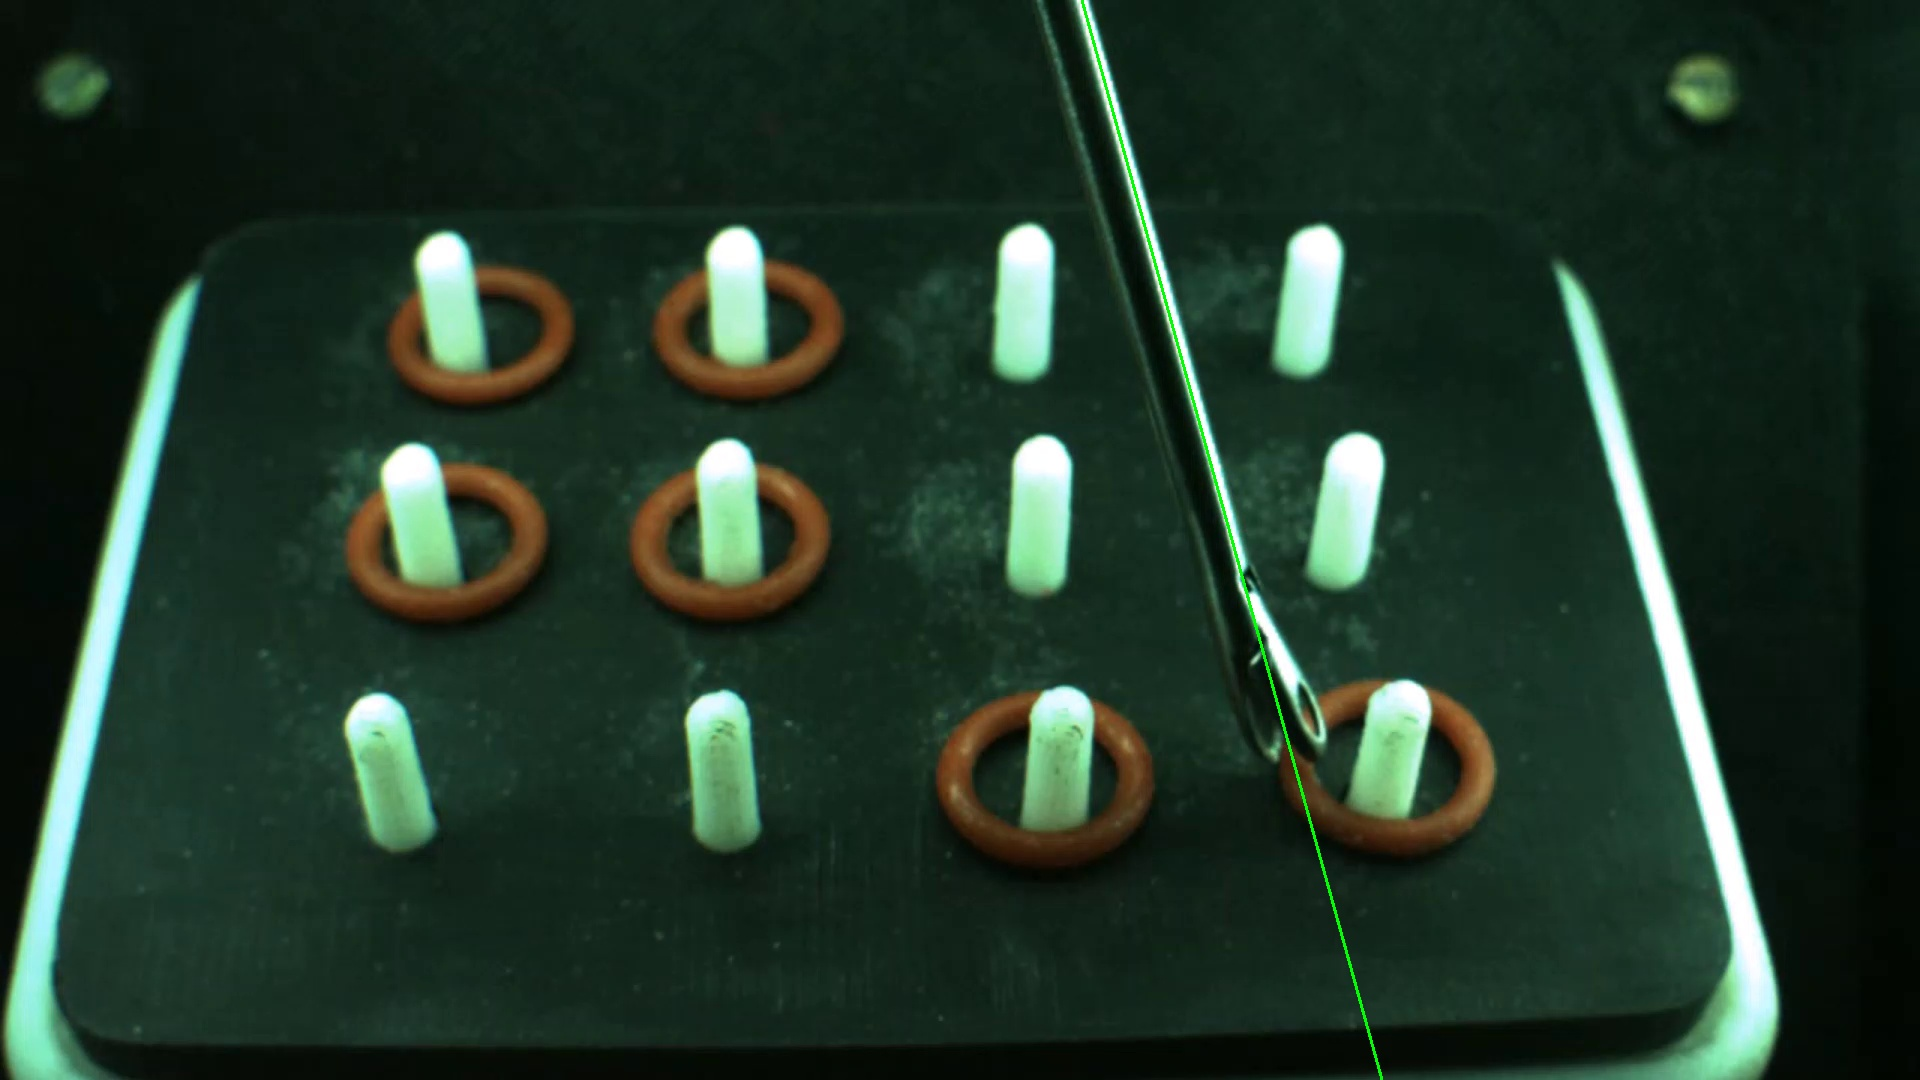
\includegraphics[width=0.6\linewidth]{results/frames/1_final.jpg}

\caption{Processing stages for Video 1 showing input frame, foreground mask, cleaned image, detected edges, and final medial axis.}
\label{fig:pipeline1}

\end{figure}

Similar behavior was observed for the other videos. 
The pipeline was able to detect the tool edges across multiple frames. 
The medial axis remained aligned with the center of the tool as it moved and rotated.

Some small fluctuations were observed when noise appeared in the mask or edges. 
However, the morphological cleaning stage reduced most of these artifacts.

Overall, the pipeline was able to detect the main structure of the surgical tool and estimate its medial axis in the tested videos.


\section{Conclusion}

In this work, a computer vision pipeline was implemented to detect the medial axis of a moving tool in video sequences. 
The approach combined background subtraction, morphological processing, edge detection, and a custom implementation of the 
Hough Line Transform.

The experimental results show that the algorithm can reliably detect the tool edges and compute a stable medial axis across 
multiple video frames. This method can serve as a foundation for further tasks such as object tracking, pose estimation, 
or robotic manipulation.


\begin{thebibliography}{99}

\bibitem{yt_cv_course}
Computer Vision Course Playlist,
\url{https://www.youtube.com/playlist?list=PLo_PZo4fbNrAegE-q9pmNWj95Cq9CRBDZ}

\bibitem{yt_opencv_video}
OpenCV Python Tutorial Video,
\url{https://www.youtube.com/watch?v=P4Z8_qe2Cu0&t=7204s}

\bibitem{opencv_docs}
OpenCV Python Documentation,
\url{https://docs.opencv.org/4.x/d6/d00/tutorial_py_root.html}

\bibitem{gfg_opencv}
GeeksforGeeks OpenCV Python Tutorial,
\url{https://www.geeksforgeeks.org/python/opencv-python-tutorial/}

\end{thebibliography}

\end{document}